
\section{Objects specification}
\label{sec:objects}


Generally speaking the code will be organized around roughly three object type categories involved in the structure of the new HOPS. These are as follows:

\begin{enumerate}
 \item Meta Data Containers: These serve to store small quantities of station and baseline metadata associated with an observation of disparate types.
 \item Array Containers: These serve to organize large n-dimensional arrays of a single data type (e.g. visibility data and correction/calibration table data). 
 \item Data Operators: These evaluate a function or perform some transformation on a given data container. Their operation is configurable via a set of externally defined parameters, while their application to any particular data set can be made conditional by a set of filters.).
\end{enumerate}

\subsection{Data Containers}

The existing HOPS3 code base relies on a fixed number of \texttt{C} structs to organize and present the data related to an observation. The strict memory layout of these structures has the advantage of making them cross-machine compatible, which is necessary since these structures are also used as the core components of the Mark-4 I/O library. However, a notable disadvantage of this rigid design is the degree of difficulty encountered in making changes to the existing data structures, or adding new data types in order to accommodate additional information which was not originally envisioned at the time the library was written. To make the data structures more flexible we intend to decouple the in-memory data layout from the file I/O, so they do not necessarily need to be byte-for-byte copies.

\subsubsection{Meta-Data Containers}

In a strictly typed language such as \texttt{C}, flexible data structures have a high degree of code overhead, not only in the management of dynamic memory allocation, but more severely in the conversion of data types and typecasting. To ameliorate this we propose to exploit \texttt{C++11}'s variadic template mechanism, which allows for the transformation of type-agnostic class lists into concrete class types or hierarchies at compile time. This makes it possible to store disparate types (so long as the complete set of types is known at compile time) within in the same object that are indexed and can be retrieved by the same type of key (e.g. a name string). Listing~\ref{lst:metaobjects} gives a condensed example of the preliminary version of the template base class for a meta-data container (with detailed functionality removed).

\lstinputlisting[language=C++,float=h!,label={lst:metaobjects},caption=Meta-data object template classes for multi-type maps.]{code/metadata-objects.hh}

To the extent possible, the in-memory meta-data structures should be classes which provide access via a key-value pair mechanism so as to avoid exposing the private internal storage layout to the routines needing access to subsets of the data. This retrieval mechanism also has the benefit of completely decoupling the compile
time structure of the data containers from the data they need to hold at runtime. A key:value interface is trivially available via the STL std::map template class,
so there is no need to expend effort on a native implementation. Moreover this sort of interface should also make conversion of these data structures into widely accessible formats such as JSON or python dictionaries possible for data export to external software.

\subsubsection{N-Dimensional Array Containers}

We propose the following basic set of class templates be used to construct most in-memory objects used for the manipulation of correlated observation data and its associated station data:
\begin{enumerate}
 \item ScalarContainer - encapsulates scalar-like data 
 \item VectorContainer - encapsulates vector-like data
 \item TableContainer - encapsulates rank-N tensor-like data with associated axes (vector)
\end{enumerate}
These template classes are to serve as a simple wrapper around the management of the raw memory needed to store a data item and keep track of its associated unit(s), 
and (if applicable) the values associated with the axes along each dimension and their units.

Listing \ref{lst:objects} gives a brief sketch of the preliminary class template implementation for these data container objects, while listing \ref{lst:visib} gives a simple example of what template declaration of an object storing visibility data from an observation over single baselines and polarization products might look like.
A graphical representation of a TableContainer is shown in Figure~\ref{fig:table-container}.

\lstinputlisting[language=C++,float=h!,label={lst:objects},caption=Data object templates]{code/data-objects.hh}

\lstinputlisting[language=C++,float=h!,label={lst:visib},caption=Visibility object type]{code/visibilities.hh}


\begin{figure}[h!]
  \begin{center}
  \captionsetup{width=0.7\linewidth}
  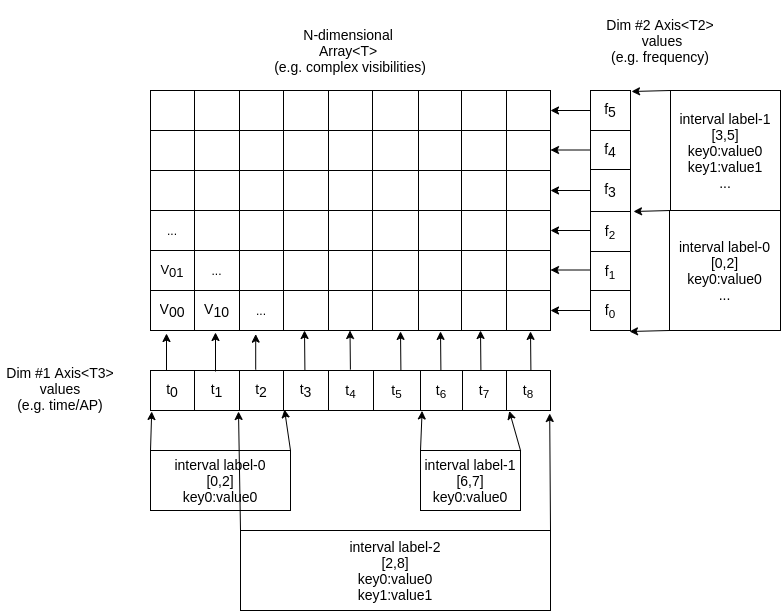
\includegraphics[width=0.75\textwidth]{fig/data-container-baseline.png}
    \caption{A graphical representation of a TableContainer. This class is composed of an N-dimensional array, coupled with axes to provide coordinate values
    along each dimension. The axes themselves allow for arbitrary intervals to be labelled by key:value pairs in order to allow for local look-up of filter data.
    For example, along the frequency axis, the interval labels may be channel or sampler names among other possibilities. Furthermore, the interval and associated
    labels will be stored in an interval-tree structure to allow for fast bi-directional lookup of data indices $\leftrightarrow$ data labels.}
    \label{fig:table-container}
\end{center}
\end{figure}

\subsection{Data operators}

The data operator classes are meant to organize the mathematic manipulations which are to be performed on the data containers. For example, many of the operations performed in the existing HOPS3 code-base (such as the application of a priori phase calibration) are relatively trivial linear transformations applied to the visibility data. However, they are currently intertwined with a large amount of control logic which obscures the basic data pathway (e.g see postproc/fourfit/norm\_fx.c)
Most unary or binary operations that are to applied to visibility or other data residing in TableContainers such as scaling, multiplication, transposition, summation, Fourier transformation, etc. will be made available as individual classes inheriting from the same interface. A uniform class interface will allow these data operators to be composed or modified to create more complicated composite operators or strung together to accomplish data pipelines of arbitrary complexity. An additional advantage of encapsulating individual operations is that any SIMD parallel-processing extension used to accelerate data processing can be made opaque to the user.

Listing \ref{lst:operators} gives a brief sketch of the class templates generalizing the data operators. The common inheritance from the base class \texttt{MHO\_DataOperator} allows them all to be stored in an common container so that once they are configured and initialized they may be retrieved
and executed in the appropriate order. It is expected that the vast majority of the data operators will be unary, requiring only their own configuration 
parameters and the data container upon which they operate as inputs, but we will also support binary operators accepting two data containers, an example
of which is the application of a pre-constructed calibration table to a new data set.

One aspect of the data operators which is not yet detailed here is a notion of what pieces of meta-data each operator may need in order to complete its function.
While these meta-data items could be exposed via external setter/getters, a more preferable option which would preserve encapsulation would be for each operator
to define an internal schema, listing the keys and type of the parameters it needs to retrieve from the meta-data multi-type map container. 
In addition, a mechanism for filtering operations (e.g. if station = Xx, then apply this operator) also needs to be established independent of the
previous control-block structure of HOPS3.

\lstinputlisting[language=C++,float=h!,label={lst:operators},caption=Data operator template classes.]{code/data-operators.hh}
